\documentclass[12pt, %
openright, 
oneside,
%twoside, %TCC: Se seu texto tem mais de 100 páginas, descomente esta linha e comente a anterior
a4paper,
english,   % hifenização do abstract
brazil]{facom-ufu-abntex2}

\usepackage{mathptmx} % fonte Times New Roman no texto e na matemática (NBR 14724)
\usepackage{graphicx}
\graphicspath{{figuras/}{pictures/}{images/}{./}}

% Floats: parâmetros menos rígidos para que tabelas e figuras fiquem
% próximas do texto que as referencia, em vez de adiadas em cascata.
\renewcommand{\topfraction}{0.85}
\renewcommand{\bottomfraction}{0.6}
\renewcommand{\textfraction}{0.1}
\renewcommand{\floatpagefraction}{0.75}

\newcommand{\blue}[1]{\textcolor{blue}{#1}}
\newcommand{\red}[1]{\textcolor{red}{#1}}


\autor{Matheus Oliveira} %TCC
\data{2026}
\orientador{Professor Renan Gonçalves Cattelan} %TCC
%\coorientador{Algum?} %TCC

% ---
% Informações de dados para CAPA e FOLHA DE ROSTO
% ---

\titulo{Desenvolvimento de um aplicativo para auxiliar
atividades de estudo} %TCC

\hypersetup{%
  pdftitle={Desenvolvimento de um aplicativo para auxiliar atividades de estudo},
  pdfauthor={Matheus Oliveira},
  pdfkeywords={aprendizagem ativa}{repetição espaçada}{procrastinação}{local-first}{extensão de navegador}{sincronização}} %TCC

\begin{document}
\frenchspacing
% NBR 10520:2023: citações entre parênteses com inicial maiúscula — (Autor, 2010)
\citeoption{opcoes-nbr10520-2023}

% ----------------------------------------------------------
% ELEMENTOS PRÉ-TEXTUAIS
% ----------------------------------------------------------
%\pretextual
\imprimircapa
\imprimirfolhaderosto


% ---
% Inserir folha de aprovação
% ---
%
% \includepdf{folhadeaprovacao_final.pdf} %TCC: depois de aprovado o trabalho, descomente esta linha e comente o próximo bloco para incluir scan da folha de aprovação.
%
%%As seções dedicatória, agradecimento e epígrafe não são obrigatórias.
%%Só as mantenha se achar pertinente.

\begin{dedicatoria}
   \vspace*{\fill}
   \centering
   \noindent
   \textit{A todos que não puderam estudar porque tiveram de trabalhar ---\\
   o mundo deve muito a vocês.}
   \vspace*{\fill}
\end{dedicatoria}

% ---
% Agradecimentos
% ---
\begin{agradecimentos}
Agradeço, primeiramente, ao professor Renan Gonçalves Cattelan: sem a sua
resiliência e agilidade, nada disto seria possível. Aos professores Pedro
Frosi Rosa, Bruno Augusto Nassif Travençolo, Rodrigo Sanches Miani e Henrique
Coelho Fernandes, que me forneceram uma base sólida para o meu crescimento
profissional --- e a todos os mestres, o meu muito obrigado.

À minha família: meus pais, Marlene Onofre de Oliveira e Berto José Carlos
de Oliveira, e minha avó, Floripes de Oliveira Souza França --- talentos que
infelizmente não tiveram a oportunidade de estudar, mas que são pessoas
extremamente inteligentes e batalhadoras, e que me fazem sentir orgulho
todos os dias da minha vida. Ao meu irmão, Thiago Vinícius Onofre de
Oliveira, e à minha noiva, Ana Carolina Oliveira Sousa, que me apoiaram
durante toda a graduação --- em especial a minha noiva, também pelo apoio na
concepção deste trabalho. Muito obrigado; amo todos vocês.

Por fim, a Gustavo de Almeida Ribeiro, mais conhecido pelo nome artístico
Black Alien, em especial pela música ``Carta pra Amy'', que me acompanhou
todos os dias, nos momentos difíceis, entre o início e o fim deste trabalho.
\end{agradecimentos}
% ---

% ---
% Epígrafe
% ---
\begin{epigrafe}
    \vspace*{\fill}
	\begin{flushright}
		\textit{``Em algum lugar, algo incrível está esperando para ser descoberto.''}\\
		--- Sharon Begley, sobre o trabalho de Carl Sagan
	\end{flushright}
\end{epigrafe}


\begin{resumo}
Este trabalho apresenta o desenvolvimento de um ecossistema de ferramentas de apoio ao estudo, 
composto por uma extensão para o navegador Google Chrome e uma interface de linha de comando (CLI),
cujo objetivo é auxiliar o estudante a manter consistência em suas atividades acadêmicas do dia a dia.
A solução integra, em um fluxo unificado de calendário, tarefas priorizadas e cartões de memorização (\textit{flashcards}), 
técnicas com eficácia sustentada pela literatura: repetição espaçada, anotações estruturadas e estratégias de organização e planejamento derivadas 
da terapia cognitivo-comportamental para adultos com déficit de atenção. Diferentemente das ferramentas predominantes,
centradas em servidores, o sistema adota uma arquitetura \textit{local-first}: todos os dados são registrados em arquivos no dispositivo do usuário, na forma de um log imutável de eventos, e a sincronização entre dispositivos ocorre pela troca explícita desses eventos com um serviço de sincronização minimalista. Essa decisão garante operação integralmente \textit{offline}, propriedade dos dados pelo usuário e longevidade da informação, ao custo de maior complexidade nos clientes --- compromisso analisado ao longo do trabalho. O texto discute os fundamentos cognitivos e comportamentais que orientaram cada funcionalidade, as decisões arquiteturais e a implementação de um protótipo funcional.

\textbf{Palavras-chave}: aprendizagem ativa; repetição espaçada; procrastinação; \textit{local-first}; extensão de navegador; sincronização. %TCC:
\end{resumo}

% ---
% Abstract (resumo em língua estrangeira, NBR 14724)
% ---
\begin{resumo}[Abstract]
\begin{otherlanguage*}{english}
This work presents the development of an ecosystem of study-support tools,
composed of a Google Chrome browser extension and a command-line interface
(CLI), whose goal is to help students maintain consistency in their everyday
academic activities. The solution integrates, in a unified flow of calendar,
prioritized tasks, and flashcards, techniques with sustained efficacy in the
literature: spaced repetition, structured note-taking, and organization and
planning strategies derived from cognitive-behavioral therapy for adults with
attention deficit. Unlike the predominant server-centric tools, the system
adopts a local-first architecture: all data is recorded in files on the
user's device, in the form of an immutable event log, and synchronization
across devices happens through the explicit exchange of these events with a
minimalist synchronization service. This decision ensures fully offline
operation, user ownership of the data, and information longevity, at the cost
of greater client complexity --- a trade-off analyzed throughout this work.
The text discusses the cognitive and behavioral foundations that guided each
feature, the architectural decisions, and the implementation of a functional
prototype.

\textbf{Keywords}: active learning; spaced repetition; procrastination;
local-first; browser extension; synchronization.
\end{otherlanguage*}
\end{resumo}

% ---

% ---
% inserir lista de ilustrações
% ---
\pdfbookmark[0]{\listfigurename}{lof}
\listoffigures*
\cleardoublepage
% ---

% ---
% inserir lista de tabelas
% ---
\pdfbookmark[0]{\listtablename}{lot}
\listoftables*
\cleardoublepage
% ---



% ---
% inserir lista de abreviaturas e siglas
% ---
% ---

%% ---
%% inserir lista de símbolos, se for adequado ao trabalho. %TCC:
%% ---
%\begin{simbolos}
%  \item[$ \Gamma $] Letra grega Gama
%  \item[$ \Lambda $] Lambda
%  \item[$ \zeta $] Letra grega minúscula zeta
%  \item[$ \in $] Pertence
%\end{simbolos}
%% ---


% ---
% inserir o sumario
% ---

\pdfbookmark[0]{\contentsname}{toc}
\tableofcontents*
\cleardoublepage
% ---





% ----------------------------------------------------------
% ELEMENTOS TEXTUAIS
% ----------------------------------------------------------
\textual


% ----------------------------------------------------------
% Introdução
% ----------------------------------------------------------

\chapter[Introdução]{Introdução}

\section{Contextualização do Trabalho}
A tecnologia é uma aliada fundamental no processo de aprendizagem, sendo crescente, nos últimos anos, o uso de ferramentas e aplicações que auxiliam os estudantes a reter informações e planejar suas atividades acadêmicas. Contudo, apesar da abundância de aplicativos e plataformas direcionados à produtividade e ao estudo, a busca por soluções acessíveis de aprendizagem ativa, voltadas a minimizar a procrastinação, ainda constitui uma demanda importante.

Aprender algo novo é desafiador para o cérebro. Nesse contexto, a aprendizagem ativa, fundamentada em metodologias que promovem o engajamento e a participação efetiva do aluno, tem se destacado como alternativa à abordagem tradicional de ensino. Técnicas que estimulam a autonomia e a organização, como a criação de \textit{flashcards}, contrubuí para a prática da repetição espaçada e fortalece a consolidação do conhecimento. Paralelamente, o estudo dos aspectos cognitivos envolvidos na memória e na atenção --- especialmente à luz do modelo de processamento de informação humano, que compreende os subsistemas dos sentidos, da memória e do processamento --- permite identificar fatores críticos que comprometem o rendimento acadêmico, como a procrastinação.

\section{Problema e Justificativa}
Enquanto algumas ferramentas especializam-se na criação de \textit{flashcards} e outras concentram-se na gestão de tarefas, observa-se a ausência de soluções que integrem esses recursos de forma coesa, fundamentadas em princípios da aprendizagem ativa e da organização cognitiva. Ademais, as ferramentas existentes dependem, em sua maioria, de conectividade constante e mantêm os dados do estudante em servidores de terceiros, o que compromete tanto o uso em contextos sem internet quanto a longevidade e a propriedade dessas informações.

Essa lacuna motivou o desenvolvimento da aplicação proposta, concebida para reunir funcionalidades voltadas ao planejamento, à memorização e ao enfrentamento da procrastinação. A aplicação, nomeada \textbf{Procrastina Não} (a escolha do nome é justificada na Seção~\ref{sec:visao-geral}), funciona de forma integrada a partir de uma extensão de navegador e uma interface de linha de comando, combinando planejamento, controle da procrastinação e técnicas de memorização sobre uma arquitetura \textit{local-first}, na qual os dados residem em arquivos no dispositivo do usuário e a sincronização entre dispositivos é explícita, proporcionando um suporte amplo ao estudante de forma acessível.

\section{Objetivos}

\subsection{Objetivo geral}
O objetivo geral do estudo consistiu em desenvolver um ecossistema de ferramentas de apoio aos estudos baseado em princípios de aprendizagem ativa, arquitetura \textit{local-first} e estratégias cognitivas voltadas à organização da rotina acadêmica.

\subsection{Objetivos específicos}
Os objetivos específicos foram os seguintes:
\begin{alineas}
  \item analisar os fatores que favorecem a procrastinação no ambiente acadêmico e as estratégias comportamentais de organização e planejamento --- em especial as derivadas da terapia cognitivo-comportamental --- capazes de mitigá-la;
  \item investigar metodologias de estudo que promovam a retenção e a recuperação eficaz da informação, com ênfase na repetição espaçada e nos métodos de anotação Cornell e Feynman;
  \item avaliar a aplicabilidade de modelos cognitivos, como o modelo de processamento de informação humano, e de arquiteturas de software \textit{local-first} na estruturação da solução;
  \item desenvolver um protótipo funcional composto por uma extensão para navegador e uma interface de linha de comando, fundamentado nos princípios identificados na revisão da literatura.
\end{alineas}

A pesquisa caracteriza-se como aplicada, com abordagem qualitativa e objetivo exploratório. Inicialmente, realizou-se pesquisa bibliográfica, com levantamento e análise da literatura sobre aprendizagem ativa, procrastinação, processos cognitivos e arquiteturas \textit{local-first}, com a finalidade de identificar os princípios que fundamentam a solução proposta e as decisões arquiteturais incorporadas ao protótipo. Em seguida, adotou-se o método \textit{Design Science Research} (DSR) para orientar a concepção, o desenvolvimento e a implementação do protótipo funcional. O DSR é o método indicado quando o produto da pesquisa é um artefato: fundamenta a construção de soluções para problemas reais e avalia o artefato pelo desempenho frente ao problema que o motivou \cite{Dresch2015}.

Em um cenário de crescente transformação digital da educação, a aplicação oferecida não pretende substituir métodos tradicionais de ensino, mas complementá-los por meio da incorporação de práticas respaldadas pela literatura sobre aprendizagem e memória, favorecendo que o estudante desenvolva autonomia para ``aprender a aprender'' \cite{EducationAppDevelopmentNeedsTpBeInformedByNeuroscience}. A principal contribuição deste trabalho é propor e implementar um artefato computacional que integra técnicas de aprendizagem ativa, estratégias de enfrentamento da procrastinação e uma arquitetura \textit{local-first}, oferecendo uma alternativa às soluções tradicionais baseadas em armazenamento centralizado.

O trabalho está organizado em quatro capítulos, estruturados de modo a atender aos objetivos da pesquisa. O Capítulo 2 fundamenta o trabalho: caracteriza a procrastinação nos estudos, apresenta as estratégias comportamentais derivadas da terapia cognitivo-comportamental, os métodos de anotação estruturada e recuperação ativa que embasam os \textit{flashcards}, os princípios de interação humano-computador que orientaram a interface e os trabalhos relacionados, evidenciando a lacuna que a aplicação ocupa. O Capítulo 3 detalha o desenvolvimento do sistema, abrangendo a visão geral dos componentes, os requisitos derivados das estratégias fundamentadas, as decisões arquiteturais \textit{local-first}, a metodologia de desenvolvimento guiado por testes e a implementação do protótipo. Por fim, o Capítulo 4 apresenta as conclusões, discutindo os resultados alcançados e indicando possíveis direções para trabalhos futuros.

\section{Declaração de uso de inteligência artificial generativa}
\label{sec:declaracao-ia}

Em conformidade com o Código de Conduta para pessoas autoras de publicações
da Sociedade Brasileira de Computação (SBC)\footnote{Disponível em:
\url{https://sol.sbc.org.br/index.php/indice/conduta}.}, declara-se que este
trabalho utilizou a ferramenta de inteligência artificial generativa Claude
(Anthropic) como apoio em três frentes: na redação e na revisão do texto dos
capítulos, a partir de textos rascunho e com decisões e direcionamento do autor; no
apoio à implementação do código e dos testes do protótipo; e na formatação
do documento em \LaTeX. A concepção do sistema, as decisões de projeto e de
arquitetura, a seleção da fundamentação teórica e a aceitação de cada trecho
gerado são do autor, que revisou integralmente o texto e o código e assume a
responsabilidade por todo o conteúdo do trabalho.

%TCC:
\chapter{O uso da tecnologia para reduzir a procrastinação nos estudos e auxiliar no processo de aprendizagem}
\label{cap:fundamentacao}

A procrastinação, que pode ser definida como o ato de fazer uma atividade
contraproducente, demorada e sem necessidade, que causa o adiamento de tarefas
importantes, está presente na rotina da maioria dos estudantes universitários:
estimativas apontam que de 30\% a 60\% dos graduandos relatam postergar
regularmente o estudo para provas, a escrita de trabalhos e as leituras
semanais \cite{AcademicProcrastinationInCollegeStudents}. O hábito de
procrastinar, além de atrapalhar o rendimento acadêmico e a qualidade de vida,
compromete a atenção na hora do estudo, o que prejudica a retenção do
conhecimento e dificulta a recuperação da memória nas provas e atividades
acadêmicas \cite{AcademicProcrastinationInCollegeStudents}.

Do ponto de vista neuropsicológico, a procrastinação está associada a déficits
no gerenciamento de metas e na autorregulação. Pesquisas de
\citeonline{GeneticRelationsAmongProcrastination} sugerem que fatores
genéticos influenciam a predisposição à procrastinação, especialmente em
indivíduos com menor capacidade de controle inibitório e planejamento. Esse
padrão reflete uma tensão entre sistemas cognitivos: o sistema límbico
(associado a recompensas imediatas) e o córtex pré-frontal (responsável pelo
planejamento e pela tomada de decisões racionais).

Assim, quando atividades acadêmicas são percebidas como complexas ou de
retorno tardio, o cérebro costuma priorizar estímulos mais gratificantes no
curto prazo, como redes sociais ou entretenimento. Experimentos
comportamentais, inclusive com animais, corroboram essa dinâmica: o estudo de
\citeonline{Mazur1996} demonstrou que até mesmo pombos tendem a adiar tarefas
que demandam esforço prolongado, optando por recompensas menores, porém
imediatas. Esse achado reforça a ideia de que a procrastinação não é
exclusivamente humana, mas sim um mecanismo ligado à economia de energia.

Para mitigar esse comportamento, estratégias baseadas em fragmentação de
tarefas têm se mostrado eficazes. Dividir atividades extensas em etapas
menores e previamente definidas reduz a percepção de sobrecarga e facilita o
engajamento inicial. Aplicativos de produtividade já incorporam essa lógica ao
permitir a organização de metas em subtarefas e prazos intermediários, a
exemplo de ferramentas de organização como o Notion e o Trello, discutidas na
Seção~\ref{sec:trabalhos-relacionados}.

Entretanto, a literatura tem mostrado que somente a disponibilidade de
ferramentas não garante a mudança de hábitos: é essencial que os sistemas se
baseiem em mecanismos de \textit{feedback} imediato e em lembretes que
fortaleçam a autorregulação \cite{EducationAppDevelopmentNeedsTpBeInformedByNeuroscience}.
A consolidação do conhecimento ocorre também nos momentos de não trabalho: um
planejamento de estudo ativo, com pausas espaçadas, otimiza a retenção na
memória e a atenção sustentada
\cite{OfflineMemoryConsolidation,BreaksAndSustainedAttention}. A prática de
recuperação constante também se mostra mais eficiente nos estudos do que a
exposição passiva ao conteúdo
\cite{EducationAppDevelopmentNeedsTpBeInformedByNeuroscience}.

Diante desse cenário, este capítulo reúne os principais referenciais teóricos
que fundamentaram as decisões de projeto adotadas no desenvolvimento da
aplicação proposta. Inicialmente, são apresentadas estratégias de organização
e autorregulação derivadas da terapia cognitivo-comportamental; em seguida,
discutem-se os métodos de anotação estruturada, recuperação ativa e repetição
espaçada que embasam o sistema de \textit{flashcards} implementado; na
sequência, abordam-se princípios da interação humano-computador utilizados
para orientar o desenvolvimento da interface; por fim, analisam-se os
trabalhos relacionados, evidenciando a lacuna que a aplicação ocupa. Em
conjunto, esses referenciais constituem a base conceitual a partir da qual
foram definidos os requisitos funcionais e as escolhas arquiteturais do
protótipo.

\section{A terapia cognitivo-comportamental como aliada dos estudos}
\label{sec:estrategias-comportamentais}

Se a procrastinação decorre, como visto, de déficits na autorregulação e no
gerenciamento de metas, uma importante aliada no enfrentamento desse problema
é a literatura clínica dedicada ao caso mais severo desses déficits: o
Transtorno de Déficit de Atenção e Hiperatividade (TDAH). Adultos com TDAH
apresentam, de forma acentuada, as mesmas dificuldades que estudantes em geral
relatam: adiamento de tarefas, gestão ineficaz do tempo, perda de materiais e
planejamento ineficiente \cite{SafrenMasteringADHD}.

Por essa razão, estratégias pensadas para essa população podem funcionar para
estudantes em geral, como um caso de \textit{design universal}: técnicas
utilizadas em casos de déficits mais graves beneficiam qualquer usuário em
momentos de fadiga ou sobrecarga cognitiva, ao reduzir o custo executivo
mental exigido pela organização. É essa a razão pela qual este trabalho adota,
como fundamento de suas funcionalidades, o programa de terapia
cognitivo-comportamental de \citeonline{SafrenMasteringADHD},
tratamento com eficácia demonstrada em ensaios clínicos randomizados e
estruturado em módulos de habilidades progressivas.

O primeiro módulo do programa --- descrito pelos autores como a fundação de
todos os demais --- estabelece uma regra central: o usuário deve manter um
único calendário, no qual registra todos os compromissos, e uma única
lista-mestra, na qual registra todas as tarefas, eliminando formas paralelas
de organização, como lembretes avulsos e listas dispersas. O objetivo é
garantir que uma única consulta diária às anotações revele tudo o que há para
fazer e, assim, eliminar a ansiedade sobre a possível existência de pendências
não registradas \cite{SafrenMasteringADHD}.

Os autores demonstram que são necessárias duas condições práticas para
sustentar o hábito de checar o calendário e as anotações: o sistema precisa
estar disponível no momento em que o compromisso é firmado, e a consulta
diária deve ser vinculada a uma rotina já existente. Sobre a lista-mestra
aplica-se a priorização por categorias: tarefas recebem classificações
conforme o nível de importância, sendo \textbf{A} para alta importância e
curto prazo, \textbf{B} para importância média e \textbf{C} para baixa
importância. O programa recomenda no máximo três ou quatro tarefas A
simultâneas, encaixadas nos blocos livres do calendário do dia, e impõe uma
regra estrita: tarefas B só devem ser iniciadas quando as tarefas A estiverem
concluídas. A regra combate um padrão típico da procrastinação: executar
primeiro as tarefas fáceis e pouco importantes, que produzem sensação de
progresso sem avanço real nas metas \cite{SafrenMasteringADHD}.

Quando uma tarefa permanece dias na lista sem ser iniciada, o programa orienta
o usuário a se perguntar o que o impede: a tarefa é grande demais? Não está
claro por onde começar? A resposta conduz à habilidade de decompor tarefas em
passos menores, cada um avaliado pelo critério ``é algo que consigo concluir
em um dia?''. Cada passo torna-se um item independente da lista-mestra,
reduzindo a percepção de sobrecarga que inibe o engajamento inicial
\cite{SafrenMasteringADHD}.

O segundo módulo refina essa decomposição com uma medida individual: a
\textit{janela de atenção} (\textit{attention span}). Em um exercício
estruturado, o usuário cronometra por quanto tempo consegue trabalhar em uma
tarefa monótona antes de se dispersar, repetindo a medição até emergir um
padrão. As tarefas passam então a ser fragmentadas em blocos dessa duração,
intercalados por pausas breves e de tempo definido. Trata-se do mesmo
princípio do método Pomodoro, porém com um refinamento importante: a duração
do bloco não é fixa em um valor arbitrário, mas ajustada à capacidade real de
cada indivíduo, que varia com o interesse, a complexidade da tarefa e o
momento \cite{SafrenMasteringADHD}.

O método da terapia cognitivo-comportamental também abrange o desenvolvimento
da habilidade de \textit{adiamento de distrações} (\textit{distractibility
delay}). Considerando o impulso identificado de o paciente abandonar a tarefa
atual quando um pensamento intrusivo surge (``preciso responder aquele
e-mail''), os autores propõem que, ao lado da tarefa, sejam mantidos um meio
de anotação rápida e um temporizador: quando a distração surge, o usuário a
registra em uma linha e retorna imediatamente à tarefa central. Ao fim do
bloco de trabalho, a lista de distrações é triada: cada item é executado,
transferido para a lista-mestra ou descartado --- e a lista temporária é então
destruída, para que não se torne mais um sistema paralelo
\cite{SafrenMasteringADHD}. A técnica busca, assim, externalizar a distração
sem interromper o foco: a confiança de que o pensamento não será perdido
remove a urgência de atendê-lo de imediato.

Complementarmente, o módulo recomenda o controle do ambiente de trabalho
(remoção de notificações e distratores visuais) e o uso de lembretes
periódicos com a pergunta ``estou fazendo o que deveria estar fazendo?'', que
interrompem episódios de dispersão não percebidos \cite{SafrenMasteringADHD}.
Vale registrar ainda que o programa dedica uma sessão específica à
procrastinação, na qual identifica mecanismos como o perfeccionismo e o
pensamento excessivamente otimista --- a crença reconfortante, porém
irrealista, de que haverá tempo suficiente no futuro (``não preciso fazer isso
hoje'') --- como fatores de manutenção do adiamento \cite{KnouseMitchell2015},
em convergência com os achados discutidos na abertura deste capítulo.

Este trabalho incorpora as estratégias da terapia cognitivo-comportamental ao
protótipo criado. Em especial, as sessões de foco registradas pelo sistema
alimentam uma estimativa da janela de atenção do usuário, que passa a calibrar
a duração sugerida dos próximos blocos de estudo --- o que auxilia no
cumprimento efetivo das demandas do usuário e combate o adiamento. Do mesmo
modo, o lembrete periódico de retorno à tarefa torna-se mensurável: o
\textit{check-in de atenção} pergunta ao estudante, na cadência que ele mesmo
define ao iniciar a sessão, se segue na tarefa, e cada resposta binária é
registrada --- convertendo a pergunta ``estou fazendo o que deveria estar
fazendo?'' em automonitoramento com dado revisável. A
Tabela~\ref{tab:estrategias-funcionalidades} resume como as estratégias do
método exposto se traduzem nas funcionalidades do sistema desenvolvido. O
mapeamento completo, incluindo os requisitos derivados de cada estratégia, é
apresentado no Capítulo~\ref{cap:desenvolvimento}.

\begin{table}[htbp]
\centering
\caption{Estratégias comportamentais e funcionalidades correspondentes (resumo).}
\label{tab:estrategias-funcionalidades}
\begin{tabular}{p{6.5cm}p{7.5cm}}
\hline
\textbf{Estratégia} & \textbf{Funcionalidade no sistema} \\
\hline
Calendário único e lista-mestra, sempre disponíveis & Base de dados local unificada, acessível pela extensão e pela CLI \\
Priorização A/B/C & Apresentação de tarefas por relevância, com limite de tarefas A \\
Quebra de tarefas em passos diários & Subtarefas vinculadas na lista-mestra \\
Janela de atenção individual & Blocos de foco com duração calibrada pelas sessões anteriores, intercalados por pausas deliberadas \\
Adiamento de distrações & Anotação rápida durante a sessão de foco, com triagem ao final \\
Lembretes de retorno à tarefa & Check-in periódico ``você está na tarefa?'' nas sessões de foco, com resposta registrada \\
\hline
\end{tabular}
\end{table}

\section{Métodos de anotação estruturada e de recuperação ativa: os \textit{flashcards} na aprendizagem}
\label{sec:anotacao-recuperacao}

A forma como o estudante registra o que aprende determina, em grande parte, o
que conseguirá reter e recuperar. Em geral, anotações meramente transcritivas
--- copiar o conteúdo tal como apresentado --- exigem pouco processamento e
produzem retenção fraca. Por outro lado, métodos de anotação estruturada
exigem que o estudante selecione, reformule ou sintetize o material, o que
possibilita que o próprio registro se converta em um ato de aprendizagem.

Nesse sentido, alguns métodos com essa proposta já foram criados. O
\textbf{método Cornell} \cite{PaukOwens2010}, por exemplo, estrutura a página
de anotações em três regiões: uma área principal, em que o conteúdo é
registrado durante o estudo; uma coluna lateral de pistas (\textit{cues}),
preenchida em seguida com palavras-chave e perguntas derivadas das notas; e um
rodapé de síntese, em que o estudante resume a página com as próprias
palavras. A revisão posterior parte da coluna de pistas com a área principal
encoberta: o estudante tenta responder às perguntas antes de conferir ---
convertendo a releitura passiva em prática de recuperação.

Por sua vez, a \textbf{técnica Feynman} complementa esse processo com um
critério de domínio: escolher um conceito e explicá-lo em linguagem simples,
como se o ensinasse a alguém leigo; identificar os pontos em que a explicação
falha; retornar à fonte para saná-los; e simplificar novamente. Embora o nome
seja de origem informal e não haja formulação canônica da técnica na
literatura acadêmica, seu mecanismo subjacente é bem documentado: a
autoexplicação \cite{Chi1994}, de modo que lacunas de compreensão que passam
despercebidas na leitura tornam-se evidentes na tentativa de reformular o que
está sendo estudado.

Ambos os métodos mencionados operacionalizam um dos achados mais robustos da
literatura de aprendizagem: a prática de recuperação (\textit{retrieval
practice}) produz retenção de longo prazo substancialmente superior à mera
releitura do material \cite{RoedigerKarpicke2006}, e seu efeito é amplificado
quando as tentativas de recuperação são distribuídas no tempo
\cite{Cepeda2006}. Esse é exatamente o fundamento da repetição espaçada
empregada pelos \textit{flashcards}.

Cabe situar a autoexplicação nesse gradiente de evidência. Na revisão
sistemática de \citeonline{Dunlosky2013}, a prática de recuperação e
a prática distribuída recebem utilidade alta; a autoexplicação e o
questionamento elaborativo (\textit{elaborative interrogation} --- responder
``por quê?'' e ``como?'' sobre o material) recebem utilidade moderada. Esse é
o papel que a explicação ocupa neste trabalho: um \emph{andaime} opcional
acoplado ao momento de recuperação, e não uma técnica autônoma. Sob esse
fundamento, o protótipo oferece a etapa de explicação em dois formatos
intercambiáveis: o campo livre da técnica Feynman e um roteiro guiado de
quatro perguntas --- composição, estrutura, origem e propósito --- inspirado
nas quatro causas aristotélicas. O roteiro é proposto como variante
estruturada do questionamento elaborativo; não há, na literatura empírica,
avaliação das ``quatro causas'' como técnica de retenção, e o texto não faz
essa alegação.

\label{sec:leitner}%
A implementação clássica da repetição espaçada em \textit{flashcards} é o
\textbf{sistema Leitner} \cite{Leitner1972}, o qual distribui cartões em
caixas numeradas, cada uma associada a um intervalo de revisão crescente ---
por exemplo, a caixa 1 é revisada diariamente; a caixa 2, a cada três dias; a
caixa 3, semanalmente. Todo cartão novo entra na caixa 1. A cada revisão, o
cartão respondido corretamente é promovido à caixa seguinte, passando a ser
revisado com menor frequência; o cartão respondido incorretamente retorna, no
esquema clássico, à caixa 1, reiniciando seu ciclo.

Dessa forma, o mecanismo busca estimular que o esforço seja concentrado
exatamente onde ele é necessário: os itens em que o estudante falha reaparecem
com frequência maior, enquanto aqueles já consolidados retornam em intervalos
progressivamente maiores. Este trabalho adota uma variante atenuada do sistema
Leitner: no erro, o cartão regride uma única
caixa, em vez de retornar à primeira posição de revisão.

Duas propriedades tornam o sistema Leitner particularmente adequado a este
trabalho. Primeiro, ele é simples e transparente: o estudante compreende por
que cada cartão apareceu, ao contrário de algoritmos de agendamento opacos.
Segundo, seu estado é integralmente derivável do histórico de revisões --- a
caixa em que um cartão se encontra é uma função pura da sequência de acertos e
erros ---, propriedade que se alinha à arquitetura de log de eventos adotada
no Capítulo~\ref{cap:desenvolvimento}: nenhum estado adicional precisa ser
armazenado ou sincronizado além dos próprios eventos de revisão.

A revisão integra-se aos blocos de foco descritos na seção anterior: ao iniciar
um bloco de estudo, o sistema enfileira os cartões vencidos --- aqueles cujas
caixas atingiram o momento de revisão, ordenados da caixa mais frágil para a
mais consolidada --- e a revisão prossegue até o temporizador do bloco soar. A
janela de atenção do estudante determina, assim, o \emph{tamanho} da sessão de
revisão, e o sistema Leitner determina o seu \emph{conteúdo}.

Em conjunto, esses métodos possuem um princípio comum: transformar o
estudante de leitor passivo em participante ativo do processo de recuperação
da informação. No sistema proposto, os métodos expostos convergem em um único
fluxo: a extensão captura o trecho grifado com a referência de origem (a área
principal do método Cornell); a triagem transforma a nota em
\textit{flashcard}, cuja frente é a pista e cujo verso é a explicação
reformulada pelo estudante com as próprias palavras (a coluna de pistas e a
técnica Feynman); e o sistema Leitner distribui as revisões nos intervalos
adequados, dentro de blocos de estudo dimensionados pela janela de atenção.
Desse modo, os fundamentos teóricos apresentados nesta seção foram
incorporados como requisitos funcionais da aplicação, orientando as decisões
de projeto adotadas no desenvolvimento do protótipo.

\section{Interação humano-computador: princípios para o desenvolvimento da interface}
\label{sec:afeto-norman}

O desenvolvimento da interface da aplicação fundamenta-se em princípios da
Interação Humano-Computador (IHC), especialmente no Modelo do Processador
Humano (MPH), proposto por \citeonline{CardMoranNewell1983}. O
modelo descreve a interação entre usuário e sistema a partir de três
subsistemas principais --- perceptual, cognitivo e motor --- e fornece um
referencial para compreender como limitações do processamento humano podem
influenciar a utilização de sistemas computacionais. Dessa forma, o MPH
constitui uma base teórica para orientar decisões de projeto que busquem
reduzir a carga cognitiva, favorecer a aprendizagem e tornar a interação mais
eficiente.

Considerando as limitações da memória de trabalho descritas pelo modelo,
tradicionalmente associadas à capacidade de processar aproximadamente sete
unidades de informação simultaneamente \cite{Miller1956}, a interface foi
concebida para minimizar a sobrecarga cognitiva durante o uso. Para isso,
foram adotados princípios clássicos de design de interfaces, como o
\textit{chunking} (agrupamento de informações), o reconhecimento em vez da
recuperação e o fornecimento de \textit{feedback} imediato ao usuário.

O princípio do \textit{chunking} consiste na organização de informações
complexas em unidades menores e mais facilmente processáveis. Na aplicação
desenvolvida, essa estratégia é empregada na divisão de metas acadêmicas em
subtarefas visuais e na organização dos conteúdos por meio de
\textit{flashcards} e etiquetas (\textit{tags}), permitindo que o estudante
concentre sua atenção em pequenas unidades de informação sem perder a visão
geral do processo de aprendizagem.

Outro princípio adotado é o do reconhecimento em vez da recuperação, segundo o
qual interfaces que apresentam opções, menus e sugestões reduzem a necessidade
de o usuário memorizar comandos ou localizar informações mentalmente
\cite{Norman1988}. Na aplicação proposta, esse princípio orienta a utilização
de menus, sugestões e elementos visuais que facilitam a navegação e reduzem o
esforço cognitivo durante o planejamento dos estudos.

Complementarmente, buscou-se fornecer \textit{feedback} imediato às ações
realizadas pelo usuário. Respostas rápidas do sistema contribuem para manter o
fluxo da interação e reduzem interrupções no processamento cognitivo, aspecto
particularmente importante em aplicações voltadas ao estudo e à manutenção do
foco. No protótipo, esse princípio materializa-se em respostas visuais
imediatas às ações do estudante e nos lembretes de retorno à tarefa exibidos
durante as sessões de foco; o elemento genuinamente adaptativo do sistema é a
duração sugerida dos blocos de estudo, calibrada pela janela de atenção medida
nas sessões anteriores.

Além desses princípios, o sistema utiliza conceitos de redes semânticas como
mecanismo para organização do conhecimento. Segundo
\citeonline{Quillian1968}, redes semânticas representam conceitos e suas relações de
forma associativa, aproximando-se da maneira como a memória humana organiza
informações. Na aplicação, essa estrutura associativa é materializada pelas
etiquetas transversais, que conectam cartões e notas de temas relacionados em
uma malha de conhecimento; a visualização gráfica dessas conexões, de forma
não linear e no estilo de ferramentas como o Obsidian, é apontada como
trabalho futuro. Essa externalização das relações reduz a carga cognitiva
intrínseca descrita por \citeonline{Sweller1988}, uma vez que parte das
relações deixa de depender exclusivamente da memória de trabalho do usuário.

Outro aspecto considerado durante o desenvolvimento foi a influência dos
fatores emocionais sobre a interação humano-computador. Conforme
\citeonline{Norman2004}, respostas afetivas positivas contribuem para uma
experiência de uso mais agradável, enquanto estímulos negativos podem
comprometer a atenção e aumentar a fadiga cognitiva. Dessa forma, buscou-se
evitar elementos que favorecessem o cansaço visual, como o uso excessivo de
cores contrastantes, bem como minimizar atrasos perceptíveis na resposta do
sistema, que tendem a gerar frustração durante a interação
\cite{MacKenzie1992}. Em contrapartida, foram incorporadas microinterações,
elementos visuais discretos e mecanismos de reforço de consistência --- a
sequência de dias de estudo e as mensagens de incentivo do mascote --- capazes
de sustentar a motivação do estudante ao longo da utilização da ferramenta.

Por fim, a acessibilidade foi considerada como um princípio transversal ao
desenvolvimento da interface. Foram adotadas estratégias como a redundância de
sinais para usuários com daltonismo --- a cor nunca é o único canal de
informação: as prioridades, por exemplo, exibem a letra da categoria além da
cor, e a interface de linha de comando respeita a convenção
\texttt{NO\_COLOR} --- e o elevado contraste entre texto e plano de fundo. A
adição de sinais sonoros complementares às notificações é apontada como
trabalho futuro. Essas escolhas contribuem não apenas para ampliar a
acessibilidade, mas também para reduzir o esforço perceptual exigido durante a
utilização cotidiana do sistema.

\section{Trabalhos relacionados}
\label{sec:trabalhos-relacionados}

As ferramentas existentes atendem a partes do problema tratado neste trabalho
e podem ser agrupadas em três categorias: organização de tarefas e projetos,
memorização por repetição espaçada e captura de conteúdo durante a navegação.

Na primeira categoria, o Notion se descreve como um espaço único para
escrever documentos, organizar conhecimento e gerenciar projetos
\cite{notion}, e o Trello reúne tarefas e quadros de trabalho em um só lugar
\cite{trello}. São ferramentas maduras de organização, mas não incorporam
mecanismos de estudo: não há repetição espaçada, prática de recuperação nem
gestão de sessões de foco. Na fronteira com a categoria seguinte, o Focus
To-Do combina o método Pomodoro com listas de tarefas \cite{PomodoroApp},
sem, contudo, vínculo com o material estudado.

Na segunda categoria, o AnkiDroid implementa a repetição espaçada de forma
madura --- ``mostrando os cartões imediatamente antes que você os esqueça''
\cite{AnkiDroid} --- e opera com dados locais, mas não organiza tarefas nem
captura conteúdo com o seu contexto de origem. O Flashcard Lab, extensão
integrada ao Google Sheets, cria cartões interativos a partir de textos de
páginas e agenda revisões por notificações do navegador; a dependência da
planilha em nuvem, porém, condiciona o estudo à conectividade.

Na terceira categoria, a extensão de Corbin, Cetinkaya e Dogan substitui a
nova aba do navegador por microconteúdo de aprendizado de idiomas ---
questões de múltipla escolha e traduções com \textit{feedback} imediato ---
transformando hábitos digitais em oportunidades de estudo. %TCC: adicionar entrada no .bib para Corbin, Cetinkaya e Dogan e citar aqui
O ReClipped, por sua vez, captura e categoriza trechos de vídeos com apoio de
processamento de linguagem natural, tornando a recuperação da informação mais
eficiente. Ambas exploram o navegador como ambiente de estudo, mas
limitam-se à captura e à exposição de conteúdo: não há calendário,
priorização de tarefas nem proteção das sessões de foco.

Às ferramentas de mercado somam-se sistemas propostos na literatura e
avaliados com estudantes. O StudiCare procrastination é uma intervenção de
terapia cognitivo-comportamental entregue por internet e celular contra a
procrastinação acadêmica: cinco módulos semanais --- psicoeducação, gestão de
tempo e definição de metas, motivação, autorregulação e prevenção de recaída
--- complementados por um diário de procrastinação e lembretes. Em ensaio
controlado randomizado com 233 universitários, o programa reduziu a
procrastinação com efeito grande em doze semanas ($d = -0{,}89$), e o
acompanhamento por um assistente digital não foi inferior ao de um psicólogo
\cite{Mutter2023StudiCare}. A adesão, porém, foi baixa --- cerca de um terço
dos participantes concluiu $80\%$ dos módulos --- e o programa é apartado do
ambiente em que a procrastinação ocorre, hospedado em plataforma central. O
Anapolo, por sua vez, é uma plataforma \textit{web} de repetição espaçada
voltada a estudantes de Direito, com agendamento pelo sistema de Leitner e
enunciados parafraseados a cada tentativa por um modelo de linguagem; em
estudo quasi-experimental com 29 estudantes, o uso da plataforma melhorou
significativamente os resultados de pós-teste ($p = 0{,}006$)
\cite{Samonte2024Anapolo}. Sua arquitetura, contudo, é inteiramente
centralizada --- servidor próprio e chamadas a uma API externa a cada
interação --- e restrita ao eixo da memorização.

A Tabela~\ref{tab:trabalhos-relacionados} consolida a comparação segundo os
eixos do problema.

\begin{table}[htbp]
\centering
\caption{Trabalhos relacionados e os eixos do problema (\textbullet{} = atende).}
\label{tab:trabalhos-relacionados}
\small
\begin{tabular}{p{3.4cm}ccccc}
\hline
\textbf{Ferramenta} & \textbf{Organização} & \textbf{Rep. espaçada} & \textbf{Captura web} & \textbf{Sessões de foco} & \textbf{\textit{Local-first}} \\
\hline
Notion & \textbullet & --- & \textbullet & --- & --- \\
Trello & \textbullet & --- & --- & --- & --- \\
Focus To-Do & \textbullet & --- & --- & \textbullet & --- \\
AnkiDroid & --- & \textbullet & --- & --- & \textbullet \\
Flashcard Lab & --- & \textbullet & \textbullet & --- & --- \\
ReClipped & --- & --- & \textbullet & --- & --- \\
StudiCare & \textbullet & --- & --- & --- & --- \\
Anapolo & --- & \textbullet & --- & --- & --- \\
\textbf{Procrastina Não} & \textbullet & \textbullet & \textbullet & \textbullet & \textbullet \\
\hline
\end{tabular}
\end{table}

Nenhuma das ferramentas cobre os eixos em conjunto: organizar o dia, capturar
com contexto, memorizar com repetição espaçada e proteger o foco são
resolvidos por aplicativos distintos, sem integração --- e, à exceção do
AnkiDroid, todos mantêm os dados do estudante em servidores de terceiros. A
mesma lacuna se repete nos sistemas da literatura: StudiCare e Anapolo
dependem integralmente de seus servidores. É
essa dupla lacuna, de integração e de propriedade dos dados, que o
\textbf{Procrastina Não} ocupa, com os requisitos derivados no
Capítulo~\ref{cap:desenvolvimento}.

\chapter{Desenvolvimento do sistema}
\label{cap:desenvolvimento}
Este capítulo descreve o desenvolvimento do sistema: a visão geral dos
componentes, os requisitos derivados das estratégias do Capítulo~\ref{cap:fundamentacao}, as
decisões arquiteturais que sustentam a operação \textit{local-first}, a
metodologia de desenvolvimento guiado por testes e a implementação dos dois
clientes, com a evidência de testes que a metodologia produz.

\section{Visão geral}
\label{sec:visao-geral}

O sistema recebeu o nome \textbf{Procrastina Não}. A escolha é deliberada: o
objetivo central da ferramenta não é uma técnica de estudo em particular, mas
sustentar a \textit{consistência} contra o seu principal adversário, a procrastinação --- o nome designa a intervenção exatamente
no momento em que ela é necessária, o impulso de adiar. A ordem coloquial
da expressão, característica do português brasileiro falado, aproxima o
sistema da voz de um colega que incentiva, em consonância com o papel do
afeto positivo na interação discutido na Seção~\ref{sec:afeto-norman}.

O sistema é um ecossistema composto por três componentes. A \textbf{extensão
para o navegador Google Chrome} é o cliente de captura: anotações rápidas,
grifos de trechos de páginas com referência de origem, criação de
\textit{flashcards}, sessões de foco com notificações e registro de distrações
durante o estudo na web. A \textbf{interface de linha de comando (CLI)},
desenvolvida em Go, é o cliente de condução do dia: exibe os próximos
compromissos e a lista diária priorizada, inicia sessões de foco com pausas
deliberadas e executa o comando de sincronização. O \textbf{serviço de
sincronização} é o componente minimalista cuja única responsabilidade é
armazenar e entregar eventos; ele não interpreta o conteúdo dos dados nem
contém regras de negócio, e sua realização proposta é um \textit{bucket} de
armazenamento de objetos, sem servidor próprio
(Seção~\ref{sub:sincronizacao}).

Os três componentes compartilham um único modelo de dados --- o log de eventos
descrito na Seção~\ref{sec:decisoes-arquiteturais} --- e nenhuma funcionalidade
de estudo depende de conectividade: a rede é exercitada exclusivamente durante
a sincronização explícita. Essa organização permite que novos clientes (como um
aplicativo móvel, previsto como trabalho futuro) sejam adicionados sem
alteração nos componentes existentes.

\section{Requisitos}
\label{sec:requisitos}

A Tabela~\ref{tab:requisitos} apresenta os requisitos funcionais (RF) e não
funcionais (RNF) do sistema, cada um rastreável à estratégia ou fundamento que
o origina. A coluna ``Cliente'' indica onde o requisito se materializa.

\begin{table}[htbp]
\centering
\caption{Requisitos do sistema e suas origens.}
\label{tab:requisitos}
\footnotesize
\begin{tabular}{p{1.2cm}p{3.4cm}p{6.6cm}p{2.2cm}}
\hline
\textbf{ID} & \textbf{Origem} & \textbf{Requisito} & \textbf{Cliente} \\
\hline
RF01 & Calendário único e lista-mestra & Registrar todos os compromissos e tarefas em uma única base local, com visão diária unificada de agenda e tarefas & Ambos \\
RF02 & Disponibilidade permanente & Capturar tarefas, notas e compromissos a partir de qualquer página (extensão) e do terminal (CLI), em uma única ação & Ambos \\
RF03 & Priorização A/B/C & Atribuir prioridade A, B ou C às tarefas; ordenar a lista diária por prioridade; limitar tarefas A simultâneas a três ou quatro; sinalizar tarefas B iniciadas antes da conclusão das A & Ambos \\
RF04 & Quebra de tarefas & Decompor tarefas em subtarefas vinculadas, cada uma tratada como item independente da lista-mestra & Ambos \\
RF05 & Janela de atenção & Registrar a duração real das sessões de foco e estimar a janela de atenção do usuário (mediana das últimas $N$ sessões), calibrando a duração sugerida dos próximos blocos de estudo & Ambos \\
RF06 & Adiamento de distrações & Capturar uma distração em uma única ação durante a sessão de foco; ao término, exigir triagem de cada item: executar, promover à lista-mestra ou descartar; a lista temporária é destruída após a triagem & Ambos \\
RF07 & Lembretes de retorno à tarefa & Perguntar ``você está na tarefa?'' durante as sessões de foco, na cadência definida pelo usuário, registrando a resposta binária para a retrospectiva & Ambos \\
RF08 & Repetição espaçada (sistema Leitner) & Criar \textit{flashcards} a partir de trechos selecionados na web, com referência de origem, e agendar revisões pelo sistema Leitner: caixas com intervalos crescentes, promoção no acerto e regressão de uma caixa no erro & Ambos \\
RF09 & Anotação estruturada & Registrar notas com campos de síntese e referência da fonte, estimulando a reformulação do conteúdo com as próprias palavras & Ambos \\
RF10 & Consistência & Exibir estatísticas de dias estudados, sessões de foco e revisões realizadas & Ambos \\
RF11 & Integração Leitner--sessão de foco & Ao iniciar uma sessão de foco de revisão, enfileirar os cartões vencidos conforme as caixas do sistema Leitner (da mais frágil para a mais consolidada) e apresentá-los até o término do bloco & Ambos \\
\hline
RNF01 & \textit{Local-first} & Operar integralmente sem rede; todos os dados residem em arquivos locais no formato do log de eventos & Ambos \\
RNF02 & Sincronização explícita & Sincronizar somente mediante comando do usuário, por troca de eventos com o serviço de sincronização & Ambos \\
RNF03 & Longevidade & Versionar os eventos; logs gravados por qualquer versão anterior do sistema permanecem legíveis & Ambos \\
\hline
\end{tabular}
\end{table}

\section{Decisões arquiteturais}
\label{sec:decisoes-arquiteturais}

A arquitetura do sistema parte do movimento \textit{local-first}
\cite{Kleppmann2019LocalFirst}, que propõe inverter a relação predominante
entre aplicativos e nuvem: em vez de o servidor deter a cópia primária dos
dados e os clientes exibirem projeções dela, a cópia primária reside no
dispositivo do usuário, e a nuvem torna-se um meio de sincronização. Dos ideais
enumerados por Kleppmann et al., três são requisitos diretos deste trabalho: o
software deve permanecer plenamente funcional sem rede, os dados devem
sobreviver ao desaparecimento de qualquer servidor, e o usuário deve deter o
controle e a propriedade das suas informações (RNF01--RNF03).

\subsection{Alternativas consideradas}

Três arquiteturas foram avaliadas. A primeira, \textbf{API centralizada}, é o
modelo convencional: o servidor mantém o estado, e os clientes realizam
requisições a cada operação. Suas vantagens são a simplicidade dos clientes e a
consistência imediata, obtida trivialmente porque há uma única cópia dos dados.
Foi descartada por violar o requisito central: sem rede não há sistema, e os
dados do estudante ficam retidos em um servidor cuja continuidade não é
garantida.

A segunda, replicação por \textbf{CRDTs} (\textit{Conflict-free Replicated
Data Types}), estrutura os dados de modo que réplicas concorrentes convirjam
automaticamente, sem coordenação. É a técnica recomendada pela literatura
\textit{local-first} para edição colaborativa em tempo real. Contudo, este
sistema é mono-usuário: as escritas concorrentes limitam-se aos dispositivos de
uma mesma pessoa, que raramente edita o mesmo dado em dois lugares no mesmo
intervalo entre sincronizações. O custo dos CRDTs --- complexidade de
implementação em duas linguagens, metadados por item e depuração difícil ---
não se justifica quando o poder que oferecem não é exercido.

A terceira alternativa, adotada, é o \textbf{log de eventos com serviço de
sincronização minimalista}: um meio-termo que preserva os ideais
\textit{local-first} com complexidade proporcional ao problema.

\subsection{O log de eventos}

Toda ação do usuário é registrada como um \textbf{evento} imutável em um log
\textit{append-only} armazenado em arquivo local. Cada evento é envelopado com
os campos: identificador único, tipo na convenção \texttt{entidade.ação} (por
exemplo, \texttt{task.created}, \texttt{card.reviewed},
\texttt{session.ended}), versão do esquema, relógio lógico, carimbo de tempo,
identificador do dispositivo de origem e carga útil específica do tipo. O
catálogo corrente define 25 tipos de evento. O log é a única fonte de verdade
do sistema.

O estado consultável --- lista de tarefas priorizada, agenda, baralhos de
\textit{flashcards}, estatísticas --- é uma \textbf{projeção}: uma função pura
que recebe a sequência de eventos e produz o estado corrente. Cada cliente
materializa as projeções de que necessita; a extensão e a CLI podem, assim,
oferecer visões distintas dos mesmos dados sem qualquer acoplamento entre si.
Nos volumes de um usuário individual, os clientes reprojetam o log a cada
consulta --- operação que permanece barata mesmo para anos de uso; quando a
escala o exigir, a pureza das projeções admite \textit{snapshots} do estado
projetado (memoização reconstruível a qualquer momento a partir do log),
otimização prevista como trabalho futuro. A posição de um cartão nas caixas do sistema
Leitner (Seção~\ref{sec:leitner}) ilustra o princípio: ela é integralmente
derivada da sequência de eventos de revisão, sem qualquer estado adicional a
armazenar ou sincronizar.

A imutabilidade do log impõe a disciplina exigida pelo RNF03: eventos gravados
nunca são alterados ou removidos, e cada tipo de evento carrega a versão do seu
esquema. Alterações de formato geram uma nova versão, e o código de projeção
mantém a capacidade de ler todas as versões anteriores.

\subsection{Sincronização}
\label{sub:sincronizacao}

A sincronização é deliberadamente simples. Cada dispositivo mantém um cursor
que indica o último evento confirmado no serviço de sincronização. Ao executar
o comando \texttt{sync}, o cliente envia os eventos locais posteriores ao
cursor e recebe os eventos, produzidos por outros dispositivos, que ainda não
possui. O serviço apenas armazena e entrega envelopes: não lê a carga útil,
não aplica regra de negócio e pode ser substituído por qualquer meio de
transporte equivalente.

Como realização do serviço, propõe-se um \textit{bucket} de armazenamento de
objetos compatível com a interface S3. A escolha decorre do próprio
protocolo: como o serviço não executa lógica alguma, um repositório de
objetos imutáveis é suficiente --- o \textit{push} grava os eventos locais
posteriores ao cursor como um objeto identificado por dispositivo e lote, e
o \textit{pull} lista e baixa os objetos ainda não vistos dos demais
dispositivos, fundindo-os no log local de forma idempotente. As
consequências são três: não há servidor próprio a desenvolver, operar ou
manter; o custo é desprezível na escala de um usuário, que produz dezenas de
quilobytes de eventos por lote; e o provedor oferece nativamente
versionamento e cópia de segurança dos objetos, reforçando o RNF03. O
\textit{bucket} pode ser provisionado na conta do próprio usuário,
preservando a propriedade dos dados defendida pelo movimento
\textit{local-first}.

A ordenação global dos eventos usa o relógio lógico de Lamport
\cite{Lamport1978}, complementado pelo carimbo de tempo físico para
desempate. Como as projeções relevantes são majoritariamente aditivas ---
criar nota, registrar revisão, concluir tarefa ---, a maioria dos eventos
comuta e a ordem de chegada é indiferente. Para o caso residual de edição
concorrente do mesmo campo em dispositivos distintos, adota-se a resolução
\textit{last-writer-wins} por campo. A idempotência é garantida pelo
identificador único: um evento recebido em duplicidade é ignorado. Essas três
propriedades --- convergência, idempotência e retrocompatibilidade --- são
objeto central da metodologia de testes descrita a seguir.

\section{Metodologia: desenvolvimento guiado por testes}
\label{sec:metodologia-tdd}

O desenvolvimento do sistema segue o \textit{Test-Driven Development} (TDD)
\cite{BeckTDD}: nenhum comportamento é implementado antes de existir um teste
que o exija. O ciclo é o clássico \textit{red-green-refactor} --- escreve-se
um teste que falha, implementa-se o mínimo que o faz passar e, então,
melhora-se a estrutura do código sob a proteção da suíte. Neste trabalho, o
TDD não é apenas uma prática de qualidade: é o instrumento que especifica o
comportamento do sistema, como descrito a seguir.

\subsection{O ciclo e o núcleo puro}

A arquitetura da Seção~\ref{sec:decisoes-arquiteturais} torna o núcleo do
sistema um conjunto de funções puras: projeções que transformam eventos em
estado, a regra de priorização A/B/C, o agendador do sistema Leitner e o
estimador de janela de atenção. Funções puras são o substrato ideal do TDD ---
os testes são rápidos, determinísticos e dispensam dublês de teste
(\textit{mocks}), pois não há entrada/saída envolvida. Todo o núcleo, tanto na
extensão quanto na CLI, é desenvolvido exclusivamente por esse ciclo.

\subsection{Vetores de conformidade entre clientes}

O maior risco de um sistema com múltiplos clientes que interpretam os mesmos
dados é a divergência semântica: a extensão (JavaScript) e a CLI (Go) poderiam
projetar estados diferentes a partir do mesmo log. A metodologia adotada
elimina esse risco tornando a especificação executável: um corpus de
\textbf{vetores de conformidade} --- arquivos JSON contendo um log de eventos
de entrada e o estado projetado esperado --- é compartilhado pelos dois
projetos, e a suíte de testes de cada cliente percorre o corpus integralmente.

O corpus é também o ponto de partida do ciclo TDD no nível de sistema: um novo
comportamento nasce como um vetor que falha em ambos os clientes
(\textit{red}) e só se considera implementado quando ambos o satisfazem
(\textit{green}). Três famílias de propriedades compõem o corpus além dos
casos funcionais: \textbf{convergência} (permutações da ordem de chegada dos
eventos produzem o mesmo estado), \textbf{idempotência} (eventos duplicados
não alteram o resultado) e \textbf{retrocompatibilidade} (logs gravados em
versões anteriores do esquema permanecem no corpus indefinidamente, garantindo
o RNF03). Um benefício direto dessa abordagem é que um futuro cliente móvel
nasce com sua especificação pronta: basta satisfazer o corpus.

\subsection{Princípios coadjuvantes}

O princípio aberto-fechado (\textit{Open-Closed Principle}) opera como
coadjuvante natural do modelo de eventos: o sistema é fechado para modificação
--- eventos gravados e seus tratadores existentes não são alterados --- e
aberto para extensão --- novas funcionalidades ingressam como novos tipos de
evento e novas projeções sobre o mesmo log. O caso ocorreu na prática: o
evento \texttt{card.explained}, que registra a explicação com as próprias
palavras durante a revisão (Seção~\ref{sec:anotacao-recuperacao}), ingressou
no catálogo com seu vetor de conformidade sem modificar o tratamento de
nenhum evento anterior --- e o padrão se repetiu em três evoluções aditivas
do catálogo desde a primeira versão do contrato: a edição e o arquivamento de
itens, as pausas registradas e o par andaime de explicação/check-in de
atenção. Campos opcionais, como o formato da explicação (\texttt{frame}) e a
cadência do check-in (\texttt{checkin\_every}), operam como pontos de
extensão: valores novos ingressam sem alterar as projeções existentes, e
clientes anteriores os ignoram por construção. Os demais princípios de projeto não são
adotados como dogma, mas emergem da própria pressão da testabilidade: as
interfaces que isolam armazenamento, relógio e notificações existem porque os
testes exigem essas costuras \cite{FreemanPryce2009} --- código difícil de
testar é o primeiro sintoma de acoplamento excessivo.

\section{Implementação}
\label{sec:implementacao}

A implementação seguiu a ordem que a metodologia impõe: primeiro a
especificação executável, depois os clientes. O catálogo de eventos, as
projeções e o protocolo de sincronização foram fixados em um documento de
especificação (\texttt{spec/SPEC.md}) acompanhado do corpus de vetores de
conformidade; em seguida foram construídos o núcleo e a interface da extensão,
em JavaScript, e por fim o núcleo e a interface da CLI, em Go --- ambos contra
o mesmo corpus.

\subsection{O TDD na prática}
\label{sub:tdd-pratica}

Cada comportamento do sistema nasceu como um vetor de conformidade em
\texttt{spec/vectors/}: um arquivo JSON com o log de entrada, o instante da
consulta e o estado projetado esperado (Figura~\ref{fig:tdd-vetor}). O corpus
conta com 33 vetores e cobre, além dos casos funcionais, as permutações de
ordem e as duplicatas que comprovam convergência e idempotência
(Seção~\ref{sec:metodologia-tdd}). O núcleo JavaScript foi escrito vetor a
vetor no ciclo vermelho--verde; o núcleo Go foi portado contra o mesmo
diretório de vetores, sem reescrever um teste, e a paridade semântica entre os
dois clientes é reverificada a cada execução das suítes. O estado corrente é
de 143 testes na extensão (Vitest) e 220 na CLI (\texttt{go test}, com detector
de condições de corrida), todos verdes (Figura~\ref{fig:tdd-suites}); no
núcleo de projeções da CLI, a cobertura de instruções é de 86\%. O corpus
também precifica o cliente móvel previsto como trabalho futuro: implementá-lo
é satisfazer os mesmos vetores.

\begin{figure}[htbp]
    \centering
    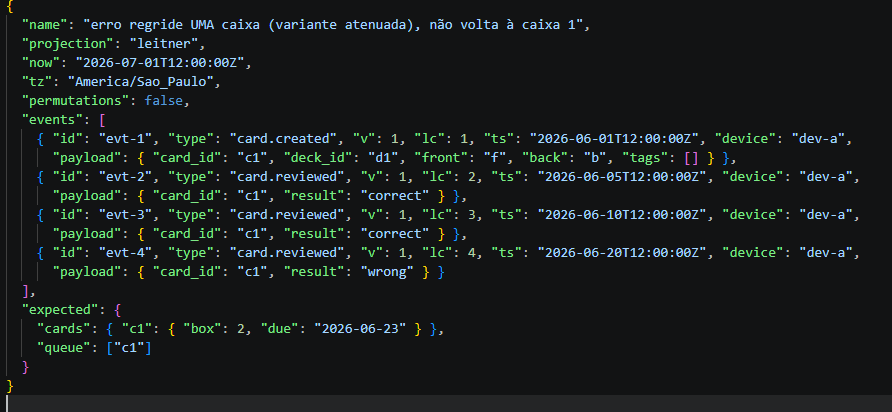
\includegraphics[width=0.95\textwidth]{figuras/tdd_vetor.png}
    \caption{Vetor de conformidade da regressão atenuada do sistema Leitner:
    dois acertos e um erro levam o cartão à caixa 2, não à caixa 1.}
    \label{fig:tdd-vetor}
\end{figure}

\begin{figure}[htbp]
    \centering
    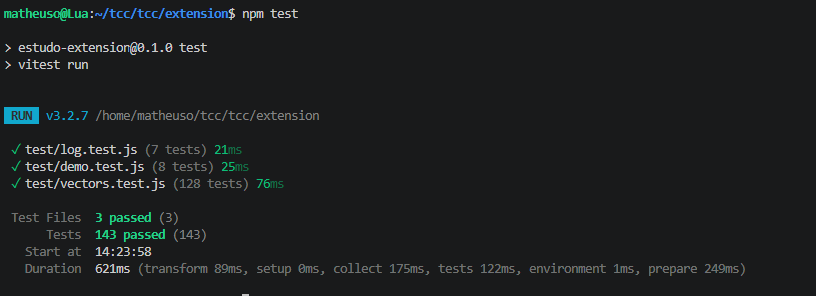
\includegraphics[width=11cm]{figuras/tdd_suite_js.png}\\[2mm]
    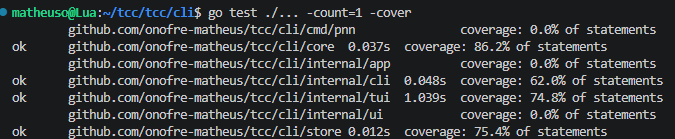
\includegraphics[width=11cm]{figuras/tdd_suite_go.png}
    \caption{As duas suítes de testes sobre o mesmo corpus de vetores: os
    testes da extensão (Vitest) e os pacotes da CLI em Go, com cobertura de
    instruções por pacote.}
    \label{fig:tdd-suites}
\end{figure}

\subsection{A extensão para o Google Chrome}
\label{sub:extensao}
A extensão foi desenvolvida com HTML5, CSS3 e JavaScript sobre a Chrome
Extensions API, na arquitetura modular do Manifest V3; o alvo é o Google
Chrome por alcance --- é o navegador de 65,92\% dos usuários
\cite{statcounter}. Não há tela de login nem requisições de autenticação: em
coerência com a arquitetura \textit{local-first}
(Seção~\ref{sec:decisoes-arquiteturais}), os dados residem no dispositivo, sob
a forma do log de eventos, e todo estado exibido é uma projeção pura desse log
lida via \texttt{chrome.storage.local}. A interface se organiza em duas
superfícies que compartilham o mesmo log local: o \textit{popup}, aberto ao
clicar no ícone da extensão, e o painel lateral (\textit{side panel}),
acionado pelo menu de contexto.

\begin{figure}[htbp]
    \centering
    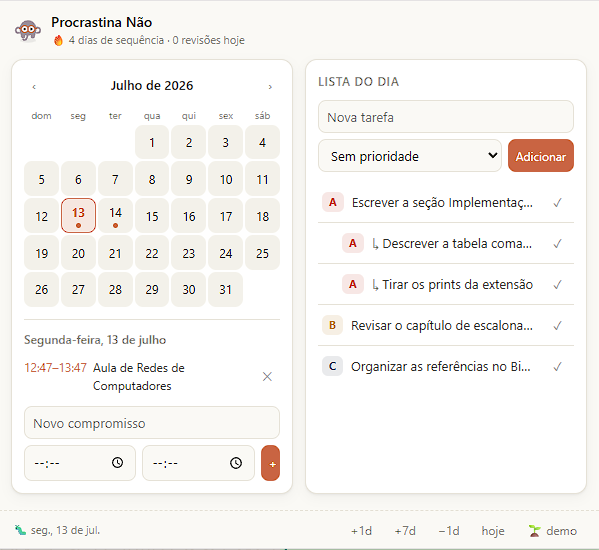
\includegraphics[width=0.85\textwidth]{figuras/tela_popup.png}
    \caption{Popup: calendário único e lista do dia com quebra de tarefas (RF01, RF03, RF04, RF10).}
    \label{fig:tela_popup}
\end{figure}

O \textit{popup} (Figura~\ref{fig:tela_popup}) reúne a agenda e as tarefas em uma única visão diária, materializando o calendário único e a lista-mestra (RF01). O cabeçalho exibe a sequência de dias estudados e o total de revisões do dia, realimentando a consistência. À esquerda, um calendário mensal navegável marca com um ponto os dias que têm compromissos; ao selecionar um dia, seus compromissos são listados por horário e um formulário permite registrar novos. À direita, a ``Lista do dia'' apresenta as tarefas ativas ordenadas por prioridade A→B→C (RF03), com um campo para criar tarefas e um seletor de prioridade; cada item pode ser repriorizado, concluído ou decomposto em subtarefas, mecanismo detalhado na Seção~\ref{sub:quebra-tarefas}.

\begin{figure}[htbp]
    \centering
    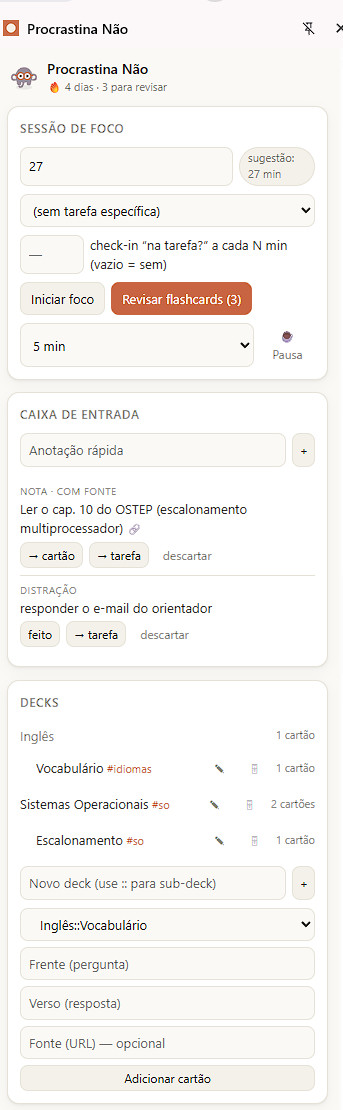
\includegraphics[width=6cm]{figuras/tela_sidepanel.png}
    \caption{Painel lateral: sessão de foco, caixa de entrada com triagem e baralhos em hierarquia (RF05, RF06, RF08, RF09).}
    \label{fig:tela_sidepanel}
\end{figure}

O painel lateral (Figura~\ref{fig:tela_sidepanel}) é exibido ao acionar ``Abrir Procrastina Não'' no menu de contexto e concentra o estudo ativo. A ``Sessão de foco'' oferece um temporizador cuja duração sugerida deriva da janela de atenção estimada a partir das sessões anteriores (RF05); durante a sessão, um campo de anotação rápida atende ao \textit{distractibility delay}, permitindo registrar a distração em uma linha e retornar imediatamente à tarefa (RF06). A ``Caixa de entrada'' lista notas capturadas na web --- inclusive pelo menu de contexto ``Anotar seleção'', que preserva a fonte (URL e título) --- e distrações pendentes de triagem, que o usuário encaminha para virar cartão, virar tarefa ou ser descartada. A seção de baralhos lista os \textit{decks} com sua contagem de cartões e oferece um formulário para criar novos baralhos e cartões, com frente, verso e fonte opcional; é também nesse painel que ocorre a revisão espaçada dos cartões, um a um, segundo o sistema Leitner (Seção~\ref{sec:leitner}; RF08, RF09, RF11). A etapa de explicação que precede a revelação do verso oferece os dois andaimes intercambiáveis da Seção~\ref{sec:anotacao-recuperacao}: o campo livre da técnica Feynman e o roteiro guiado das quatro causas.

A sessão de foco materializa também o RF07, na forma do \textbf{check-in de atenção}: ao iniciar o bloco, o estudante pode vincular a sessão a uma tarefa da lista do dia e definir uma cadência em minutos; a cada intervalo, o navegador emite uma notificação com a pergunta ``Você está na tarefa?'' --- citando a tarefa pelo nome --- e dois botões de resposta, ``sim, na tarefa'' e ``não, distraí''. A pergunta parte do \textit{service worker} da extensão, de modo que alcança o estudante mesmo com o painel fechado --- precisamente o cenário em que a dispersão passa despercebida ---, e cada resposta é gravada como evento (\texttt{checkin.logged}). A retrospectiva semanal do painel agrega os resultados na forma ``na tarefa em X de Y checagens'', transformando o lembrete periódico de Safren et al. (Seção~\ref{sec:estrategias-comportamentais}) em automonitoramento com dado revisável, e não em mera interrupção. As pausas seguem a mesma disciplina de duração definida: o estudante escolhe blocos de 5 a 25 minutos, e pausar durante uma sessão de foco a \emph{encerra} --- a pausa é um estado próprio, registrado no log, não um parêntese dentro do foco.

\subsection{Quebra de tarefas na lista do dia}
\label{sub:quebra-tarefas}
A lista do dia, exibida no \textit{popup}, materializa a estratégia de decomposição de tarefas (Seção~\ref{sec:estrategias-comportamentais}) e o requisito RF04. Cada tarefa apresenta um botão de decomposição que abre um campo em linha para registrar um passo menor; a subtarefa resultante é gravada como um evento \texttt{task.created} portando o identificador da tarefa-mãe (\texttt{parent\_id}), e nenhuma extensão do modelo de eventos foi necessária, pois o envelope já previa esse vínculo. A projeção da lista do dia continua devolvendo todas as tarefas ativas ordenadas por prioridade A→B→C; a interface, a partir desse resultado plano, reconstrói a hierarquia e apresenta as subtarefas recuadas sob a respectiva tarefa-mãe, preservando a ordem por prioridade entre irmãs. Cada subtarefa é um item independente da lista-mestra --- pode receber prioridade própria, ser concluída isoladamente e, caso a tarefa-mãe seja concluída antes, permanece visível promovida ao nível principal, de modo que nenhum passo se perca. Assim, a decomposição sugerida pela terapia cognitivo-comportamental para reduzir a percepção de sobrecarga (Seção~\ref{sec:estrategias-comportamentais}) é oferecida sem custo cognitivo adicional de navegação: o estudante fragmenta a tarefa no mesmo lugar em que a consulta.

\subsection{A interface de linha de comando}
\label{sub:cli}

A CLI foi desenvolvida em Go e distribui-se como um binário estático único,
\texttt{pnn}, sem dependências de execução: instalar é copiar um arquivo, e
nada além do sistema de arquivos é exigido em tempo de uso (RNF01). Três
bibliotecas compõem a interface: Cobra estrutura os comandos e a ajuda; Bubble
Tea implementa as sessões interativas segundo a arquitetura Elm --- o estado
da tela é atualizado por uma função pura, o que permitiu desenvolver as
sessões pelo mesmo ciclo TDD, sem terminal --- e Lipgloss aplica os estilos. A
réplica local é um arquivo \texttt{events.jsonl} no diretório
\texttt{\textasciitilde/.pnn}, um evento por linha, protegido por trava de
arquivo contra escritas concorrentes; o relógio de Lamport é derivado do maior
valor presente no log, e a fusão de eventos remotos é idempotente --- as
mesmas propriedades verificadas pelos vetores de conformidade.

A interação divide-se em dois regimes, sinalizados por cor. No modo de
organização (azul), os comandos são \textit{one-shot}: executam, imprimem e
devolvem o terminal. \texttt{pnn dia} (Figura~\ref{fig:cli-dia}) é a visão de
condução do dia --- agenda, lista A/B/C com subtarefas e a sequência de dias
estudados ---, e os itens exibidos recebem números efêmeros reutilizados pelo
comando seguinte (\texttt{pnn feito 2}, \texttt{pnn pri 3 A}). Nas sessões
imersivas a tela alterna para o modo vermelho: \texttt{pnn foco}
(Figura~\ref{fig:cli-foco}) inicia um bloco com duração sugerida pela janela
de atenção e mantém a linha de entrada permanentemente focada, de modo que
registrar uma distração custa digitá-la e teclar Enter; com
\texttt{--checkin N}, o terminal soa a cada $N$ minutos e pergunta ``você
está na tarefa?'', respondida com uma única tecla e registrada no log (RF07).
\texttt{pnn revisar} (Figura~\ref{fig:cli-revisar}) percorre a fila do
sistema Leitner, pede a explicação com as próprias palavras antes de revelar
o verso --- alternável, pela tecla Tab, entre o campo livre Feynman e o
roteiro das quatro causas (Seção~\ref{sec:anotacao-recuperacao}) --- e
encerra quando a fila acaba ou o temporizador toca. A pausa entre blocos é o
modo verde (Figura~\ref{fig:cli-pausa}) e opera como reforço de conclusão:
sessão interrompida não ganha pausa; o estudante pode, ainda, abrir uma pausa
deliberada de 5 a 25 minutos durante o foco, o que encerra a sessão ---
mesma semântica da extensão. A retrospectiva \texttt{pnn semana} agrega, por
dia, minutos de foco, pausas, revisões, motivos de interrupção e o resultado
dos check-ins (``na tarefa em X de Y''). \texttt{pnn triagem}
(Figura~\ref{fig:cli-triagem}) percorre a caixa de entrada um item por vez
--- virar cartão, virar tarefa ou descartar ---, a triagem obrigatória que
fecha o ciclo do adiamento de distrações (RF06). Toda
leitura aceita \texttt{--json}, a cor nunca é o único canal de informação e a
convenção \texttt{NO\_COLOR} é respeitada. A
Tabela~\ref{tab:cli-requisitos} consolida a correspondência entre comandos e
requisitos.

\begin{table}[htbp]
\centering
\caption{Correspondência entre comandos da CLI e requisitos.}
\label{tab:cli-requisitos}
\small
\begin{tabular}{p{3.8cm}p{7.0cm}p{2.4cm}}
\hline
\textbf{Comando} & \textbf{Comportamento} & \textbf{Requisitos} \\
\hline
\texttt{pnn dia} & Agenda do dia, lista A/B/C com subtarefas, alerta de excesso de tarefas A, sequência de dias e revisões & RF01, RF03, RF04, RF10 \\
\texttt{pnn t}, \texttt{pnn n}, \texttt{pnn c} & Captura de tarefa, nota e compromisso em uma única linha & RF02 \\
\texttt{pnn t --sub N} & Subtarefa vinculada à tarefa \texttt{N} & RF04 \\
\texttt{pnn pri N}, \texttt{pnn feito N} & Repriorização e conclusão pelos números efêmeros & RF03 \\
\texttt{pnn foco [N]} & Sessão de foco com duração sugerida pela janela de atenção, linha de captura de distrações e check-in de atenção opcional (\texttt{--checkin}) & RF05, RF06, RF07 \\
\texttt{pnn semana} & Retrospectiva semanal: foco, pausas, revisões, motivos de interrupção e check-ins agregados por dia & RF07, RF10 \\
\texttt{pnn caixa}, \texttt{pnn triagem} & Pendências de triagem; triagem item a item: virar cartão, virar tarefa ou descartar & RF06 \\
\texttt{pnn revisar [deck]} & Fila Leitner da caixa mais frágil à mais consolidada, até o temporizador tocar; explicação com as próprias palavras antes de revelar o verso & RF08, RF09, RF11 \\
\texttt{pnn carta [deck]}, \texttt{pnn deck} & Criação de cartões em série (frente, verso, fonte) e de baralhos & RF08, RF09 \\
\hline
\end{tabular}
\end{table}

\begin{figure}[htbp]
    \centering
    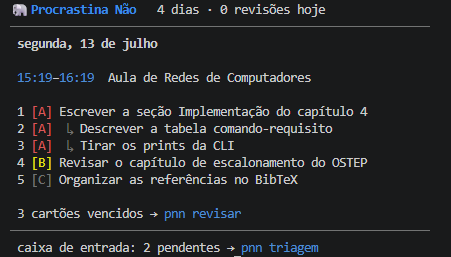
\includegraphics[width=9cm]{figuras/cli_dia.png}
    \caption{\texttt{pnn dia}: estatísticas de consistência, agenda e lista
    A/B/C com subtarefas e números efêmeros (modo azul; RF01, RF03, RF04,
    RF10).}
    \label{fig:cli-dia}
\end{figure}

\begin{figure}[htbp]
    \centering
    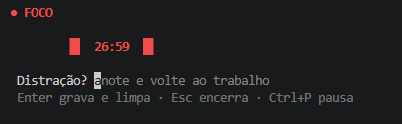
\includegraphics[width=9cm]{figuras/cli_foco.png}
    \caption{\texttt{pnn foco}: sessão de foco com duração sugerida pela
    janela de atenção (27 min) e a linha de captura de distrações sempre
    focada (modo vermelho; RF05, RF06).}
    \label{fig:cli-foco}
\end{figure}

\begin{figure}[htbp]
    \centering
    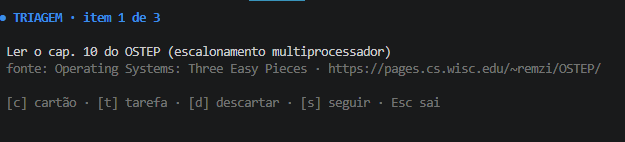
\includegraphics[width=10cm]{figuras/cli_triagem_nota.png}\\[2mm]
    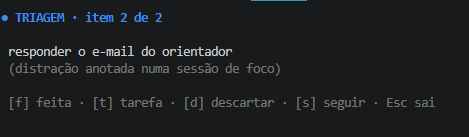
\includegraphics[width=8cm]{figuras/cli_triagem_distracao.png}
    \caption{\texttt{pnn triagem}: nota com fonte preservada e distração
    capturada em sessão de foco, triadas uma a uma (RF06).}
    \label{fig:cli-triagem}
\end{figure}

\begin{figure}[htbp]
    \centering
    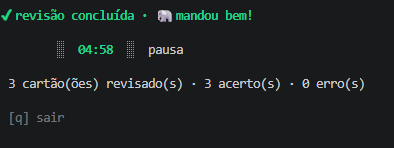
\includegraphics[width=9cm]{figuras/cli_pausa.png}
    \caption{Fim de sessão de revisão: resumo de acertos e pausa em modo
    verde --- o reforço de conclusão.}
    \label{fig:cli-pausa}
\end{figure}

\begin{figure}[htbp]
    \centering
    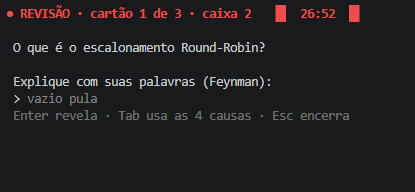
\includegraphics[width=9cm]{figuras/cli_revisar_pergunta.png}\\[2mm]
    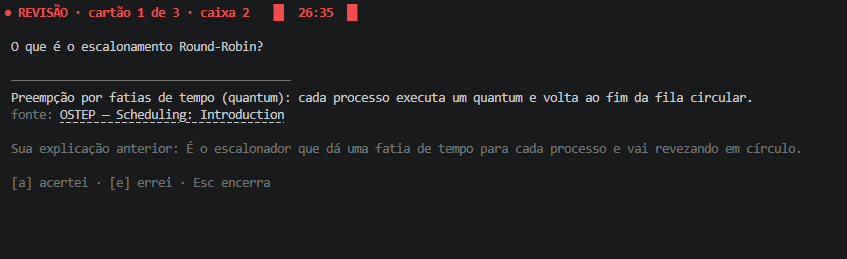
\includegraphics[width=0.95\textwidth]{figuras/cli_revisar.png}
    \caption{\texttt{pnn revisar}, antes e depois de revelar: explicação com
    as próprias palavras e, no verso, a fonte da captura em hiperlink e a
    explicação anterior reapresentada (RF08, RF09, RF11).}
    \label{fig:cli-revisar}
\end{figure}

O binário instala um segundo nome, \texttt{procrastina}, disponível também como
subcomando (\texttt{pnn procrastina}); grafias erradas comuns, como
\texttt{procastina}, são aceitas --- a intervenção não pode falhar por um erro
de digitação no momento do impulso. Executá-lo imprime a recusa --- ``Não.''
---, a sequência de dias corrente e o menor próximo passo ativo, com o comando
\texttt{pnn foco} pronto para colar (Figura~\ref{fig:cli-procrastina}): é a
materialização literal do nome do sistema, a intervenção no instante do
impulso de procrastinar. Da sincronização (RNF02), o
lado cliente está implementado e testado --- \textit{outbox}, cursor e fusão
idempotente ---; a integração com o \textit{bucket} proposto na
Seção~\ref{sub:sincronizacao} é a etapa final do desenvolvimento, discutida
no Capítulo~\ref{cap:conclusao}.

\begin{figure}[htbp]
    \centering
    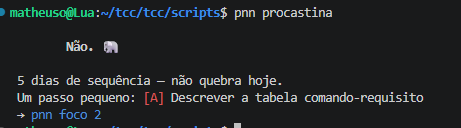
\includegraphics[width=9.5cm]{figuras/cli_procrastina.png}
    \caption{\texttt{procrastina}: a intervenção que dá nome ao sistema.}
    \label{fig:cli-procrastina}
\end{figure}

\subsection{Repositório de código e instalação}
\label{sub:repositorio}

O código-fonte completo do sistema está disponível no repositório do
trabalho\footnote{Disponível em: \url{https://github.com/onofre-matheus/tcc}.}.
A estrutura de diretórios
espelha a arquitetura: \texttt{spec/} contém a especificação
(\texttt{SPEC.md} e \texttt{CLI.md}) e o corpus de vetores de conformidade
(\texttt{spec/vectors/}); \texttt{extension/} e \texttt{cli/} contêm os dois
clientes, cada um com sua suíte de testes apontada para o mesmo corpus.

A instalação reflete o RNF01. A CLI é um binário estático: instalar é
copiá-lo para um diretório do \texttt{PATH}, e a réplica local é criada em
\texttt{\textasciitilde/.pnn} no primeiro uso --- as variáveis de ambiente
\texttt{PNN\_HOME} e \texttt{PNN\_TZ} permitem, opcionalmente, redefinir o
diretório de dados e o fuso horário. A extensão é carregada no Google Chrome
pelo modo do desenvolvedor (\texttt{chrome://extensions}), sem cadastro nem
serviço externo; a publicação na Chrome Web Store é etapa de distribuição,
não de desenvolvimento.

\chapter{Conclusão}
\label{cap:conclusao}

Este trabalho propôs, fundamentou e implementou o Procrastina Não: um
ecossistema \textit{local-first} de apoio aos estudos composto por uma
extensão para o navegador e uma interface de linha de comando, que traduz em
funcionalidades as estratégias comportamentais e cognitivas levantadas na
literatura. Este capítulo retoma os objetivos definidos na introdução,
reconhece as limitações do que foi construído e indica os desdobramentos do
trabalho.

\section{Retrospectiva}

O objetivo geral --- desenvolver um ecossistema de ferramentas de apoio aos
estudos baseado em aprendizagem ativa, arquitetura \textit{local-first} e
estratégias cognitivas de organização da rotina acadêmica --- foi atingido
por meio dos quatro objetivos específicos. O objetivo (a) foi atendido no
Capítulo~\ref{cap:fundamentacao}, que caracterizou os fatores associados à
procrastinação acadêmica e derivou da terapia cognitivo-comportamental as
estratégias de organização e planejamento que se tornaram requisitos do
sistema (Seção~\ref{sec:estrategias-comportamentais}). O objetivo (b) foi
atendido pela investigação da repetição espaçada, do sistema Leitner e dos
métodos de anotação Cornell e Feynman
(Seção~\ref{sec:anotacao-recuperacao}), cada um rastreável a um requisito
funcional na Tabela~\ref{tab:requisitos}. O objetivo (c) materializou-se nas
decisões arquiteturais do Capítulo~\ref{cap:desenvolvimento}: o modelo de
processamento de informação humano orientou a interface, e os ideais
\textit{local-first} foram realizados pelo log imutável de eventos com
projeções puras. O objetivo (d) foi cumprido com o protótipo funcional: os
dois clientes cobrem os onze requisitos funcionais e operam integralmente
sem rede.

Além do artefato, o trabalho demonstrou um método: a especificação executável
por vetores de conformidade compartilhados. O corpus de 33 vetores é
percorrido pelas suítes de ambos os clientes a cada execução, verificando
convergência, idempotência e retrocompatibilidade
(Seção~\ref{sec:metodologia-tdd}); a paridade semântica entre uma
implementação em JavaScript e outra em Go deixou de ser uma esperança de
disciplina para ser uma propriedade testada.

\section{Limitações do Trabalho}

A primeira limitação é a ausência de avaliação com usuários. A metodologia
adotada valida a correção do sistema, mas não a sua eficácia comportamental:
afirmar que o uso do Procrastina Não reduz a procrastinação ou melhora a retenção
exigiria um estudo empírico com estudantes, fora do escopo deste trabalho.

A segunda limitação, é que a sincronização não foi integrada. O lado cliente
está implementado e testado, e o transporte proposto
(Seção~\ref{sub:sincronizacao}) está especificado, mas a conexão com um
\textit{bucket} real não foi realizada; no estado atual, as réplicas da
extensão e da CLI evoluem de forma independente. As demais propriedades
\textit{local-first} não são afetadas: cada cliente é plenamente funcional
sem rede.

\section{Trabalhos Futuros}

O primeiro desdobramento é a integração da sincronização com o
\textit{bucket} S3 proposto. Como a fusão idempotente, o cursor e a
\textit{outbox} já existem e estão sob teste, o trabalho restante
limita-se ao transporte: as operações de \textit{push} e \textit{pull}
de objetos com versionamento e backup nativo.

O segundo é o cliente móvel. A metodologia adotada precifica essa extensão:
um aplicativo móvel nasce com a especificação pronta, bastando satisfazer o
mesmo corpus de vetores de conformidade que hoje governa a extensão e a CLI.

Seguem-se duas extensões de interface fundamentadas no
Capítulo~\ref{cap:fundamentacao}: o grafo de conexões entre notas e cartões,
que materializa a organização associativa do conhecimento discutida na
Seção~\ref{sec:anotacao-recuperacao}, e a personalização das notificações de
retorno à tarefa --- hoje implementadas como o check-in de atenção
(Seção~\ref{sub:extensao}) --- com sinais sonoros configuráveis pelo usuário
(Seção~\ref{sec:afeto-norman}).

Por fim, duas otimizações de armazenamento acompanham o crescimento do log:
\textit{snapshots} das projeções puras
(Seção~\ref{sec:decisoes-arquiteturais}) e a migração do log da extensão de
\texttt{chrome.storage.local} para IndexedDB, com escrita de custo constante
por evento --- passo que, adicionalmente, aproxima o núcleo JavaScript de um
empacotamento como aplicativo web progressivo para dispositivos móveis.

% ----------------------------------------------------------
% ELEMENTOS PÓS-TEXTUAIS
% ----------------------------------------------------------
\postextual


% ----------------------------------------------------------
% Referências bibliográficas
% ----------------------------------------------------------
\bibliography{abntex2-modelo-references}

%---------------------------------------------------------------------
% INDICE REMISSIVO
%---------------------------------------------------------------------

\printindex



\end{document}